\subsection{2D Poisson problem on Square - Dirichlet BC}

\begin{frame}{Problem considered} 
	\textbf{Problem statement:} Consider the Poisson problem with Dirichlet BC:
	\vspace{-5pt}
	\begin{equation*}
		\left\{
		\begin{aligned}
			-\Delta u & = f, \; &  & \text{in } \; \Omega \times \mathcal{M}, \\
			u         & =0, \;  &  & \text{on } \; \partial\Omega \times \mathcal{M},
		\end{aligned}
		\right.
		% \label{eq:Lap2D}\tag{$\mathcal{P}$}
	\end{equation*}

	\vspace{-5pt}
	with $\Omega=[-0.5 \pi, 0.5 \pi]^2$ and $\mathcal{M}=[-0.5,0.5]^2$ ($p=2$ parameters).
		
	\vspace{8pt}
	\textbf{Analytical solution :}

	\vspace{-5pt}
	\begin{equation*}
		% \label{eq:analytical_solution_Lap2D}
		u(\bm{x},\bm{\mu})=\exp\left(-\frac{(x-\mu_1)^2+(y-\mu_2)^2}{2}\right)\sin(2 x)\sin(2 y).
	\end{equation*}

	\vspace{12pt}
	\textbf{PINN training:} MLP of 5 layers; LBFGs optimizer (5000 epochs). \\
	Imposing the Dirichlet BC exactly in the PINN with the levelset $\varphi$ defined by
	$$\varphi(\bm{x})=(x+0.5\pi)(x-0.5\pi)(y+0.5\pi)(y-0.5\pi).$$
	
	\small\vspace{4pt}
	Training time : less than 1 hour on a laptop GPU.
\end{frame}

\begin{frame}{Numerical results}
	\hspace{-5pt}\begin{minipage}[t]{0.46\linewidth}
		\textbf{Error estimates :} 1 set of parameters.
		$$\bm{\mu}^{(1)}=(0.05, 0.22) $$
		\vspace{-35pt}
		\begin{figure}[H]
			\cvgFEMCorrAlldeg{images/numeric/poisson/dirichlet/cvg/FEM_case1_v1_param1.csv}{images/numeric/poisson/dirichlet/cvg/Corr_case1_v1_param1.csv}{1e-10}
		\end{figure}
	\end{minipage} \qquad \small
	\begin{minipage}[t]{0.48\linewidth}
	\end{minipage}
\end{frame}

\begin{frame}[noframenumbering]{Numerical results}
	\hspace{-5pt}\begin{minipage}[t]{0.46\linewidth}
		\textbf{Error estimates :} 1  set of parameters.
		$$\bm{\mu}^{(1)}=(0.05, 0.22) $$
		\vspace{-35pt}
		\begin{figure}[H]
			\cvgFEMCorrAlldeg{images/numeric/poisson/dirichlet/cvg/FEM_case1_v1_param1.csv}{images/numeric/poisson/dirichlet/cvg/Corr_case1_v1_param1.csv}{1e-10}
		\end{figure}
	\end{minipage} \qquad \small
	\begin{minipage}[t]{0.48\linewidth}
		\textbf{Gains achieved :} $n_p=50$ sets of parameters.
		$$\mathcal{S}=\left\{\bm{\mu}^{(1)},\dots,\bm{\mu}^{(n_p)}\right\}$$
		\vspace{-15pt}
		\begin{table}[H]
			\gainstableallq{images/numeric/poisson/dirichlet/gains/Tab_stats_case1_v1.csv}
		\end{table}

		\normalsize\centering\vspace{-20pt}
		$$N=20$$

		\vspace{-5pt}
		Gain : $\| u-u_h\|_{L^2} / \| u-u_h^+\|_{L^2}$ \\
		
		\small\vspace{8pt}
		Cartesian mesh : $N^2$ nodes.
	\end{minipage}
\end{frame}

\begin{frame}[noframenumbering]{Numerical results}
	\hspace{-5pt}\begin{minipage}[t]{0.46\linewidth}
		\textbf{Error estimates :} 1 set of parameters.
		$$\bm{\mu}^{(1)}=(0.05, 0.22) $$
		\vspace{-35pt}
		\begin{figure}[H]
			\cvgFEMCorrAlldegLine{images/numeric/poisson/dirichlet/cvg/FEM_case1_v1_param1.csv}{images/numeric/poisson/dirichlet/cvg/Corr_case1_v1_param1.csv}{1e-10}
		\end{figure}
	\end{minipage} \qquad \small
	\begin{minipage}[t]{0.48\linewidth}
		\textbf{$N_\text{dofs}$ required to reach the same error $e$ :}

		\vspace{10pt}
		\begin{table}[H]
			\centering
			\coststableallq{images/numeric/poisson/dirichlet/costs/TabDoFs_case1_v1_param1.csv}
		\end{table}
	\end{minipage}
\end{frame}

\subsection{2D Anisotropic Elliptic problem on a Square - Dirichlet BC}

\begin{frame}{Problem considered} 
	\textbf{Problem statement:} Considering an Anisotropic Elliptic problem with Dirichlet BC:
	\vspace{-5pt}
	\begin{equation*}
		\left\{
		\begin{aligned}
			-\text{div}(D\nabla u) & = f, \; &  & \text{in } \; \Omega, \\
			u         & =0, \;  &  & \text{on } \; \partial\Omega,
		\end{aligned}
		\right.
		% \label{eq:Ell2D}\tag{$\mathcal{P}$}
	\end{equation*}

	with $\Omega=[0,1]^2$ and $\mathcal{M}=[0.4, 0.6]\times [0.4, 0.6]\times [0.01,1]\times [0.1,0.8]$ ($p=4$).
	
	\vspace{8pt}
	\textbf{Right-hand side :}

	\vspace{-5pt}
	\begin{equation*}
		f(\bm{x},\bm{\mu})=\exp\left(-\frac{(x-\mu_1)^2+(y-\mu_2)^2}{0.025\sigma^2}\right).
	\end{equation*}
	
	\textbf{Diffusion matrix :} (symmetric and positive definite)
	\begin{equation*}
		D(\bm{x},\bm{\mu})=\begin{pmatrix}
			\epsilon x^2+y^2 & (\epsilon-1)xy \\
			(\epsilon-1)xy & x^2+\epsilon y^2
		\end{pmatrix}.
	\end{equation*}

	\vspace{2pt}
	\textbf{PINN training:} MLP with Fourier Features\footcite{TanSri2020} of 5 layers; Adam optimizer (15000 epochs). Imposing the Dirichlet BC exactly in the PINN with a level-set function.

	\vspace{5pt}
\end{frame}

\begin{frame}{Numerical results}
	\hspace{-5pt}\begin{minipage}[t]{0.46\linewidth}
		\textbf{Error estimates :} 1 set of parameters.
		$$\bm{\mu}^{(1)}=(0.51,0.54,0.52,0.55)$$
		\vspace{-35pt}
		\begin{figure}[H]
			\cvgFEMCorrAlldeg{images/numeric/elliptic/cvg/FEM_case3_v1_param1.csv}{images/numeric/elliptic/cvg/Corr_case3_v1_param1.csv}{1e-9}
		\end{figure}
	\end{minipage} \qquad \small
	\begin{minipage}[t]{0.48\linewidth}
	\end{minipage}
\end{frame}

\begin{frame}[noframenumbering]{Numerical results}
	\hspace{-5pt}\begin{minipage}[t]{0.46\linewidth}
		\textbf{Error estimates :} 1 set of parameters.
		$$\bm{\mu}^{(1)}=(0.51,0.54,0.52,0.55)$$
		\vspace{-35pt}
		\begin{figure}[H]
			\cvgFEMCorrAlldeg{images/numeric/elliptic/cvg/FEM_case3_v1_param1.csv}{images/numeric/elliptic/cvg/Corr_case3_v1_param1.csv}{1e-9}
		\end{figure}
	\end{minipage} \qquad \small
	\begin{minipage}[t]{0.48\linewidth}
		\textbf{Gains achieved :} $n_p=50$ sets of parameters.
		$$\mathcal{S}=\left\{\bm{\mu}^{(1)},\dots,\bm{\mu}^{(n_p)}\right\}$$
		\vspace{-15pt}
		\begin{table}[H]
			\gainstableallq{images/numeric/elliptic/gains/Tab_stats_case3_v1.csv}
		\end{table}

		\normalsize\centering\vspace{-20pt}
		$$N=20$$

		\vspace{-5pt}
		Gain : $\| u-u_h\|_{L^2} / \| u-u_h^+\|_{L^2}$ \\
		
		\small\vspace{8pt}
		Cartesian mesh : $N^2$ nodes.
	\end{minipage}
\end{frame}

\begin{frame}{Numerical results}
	\begin{figure}[!ht] \centering
		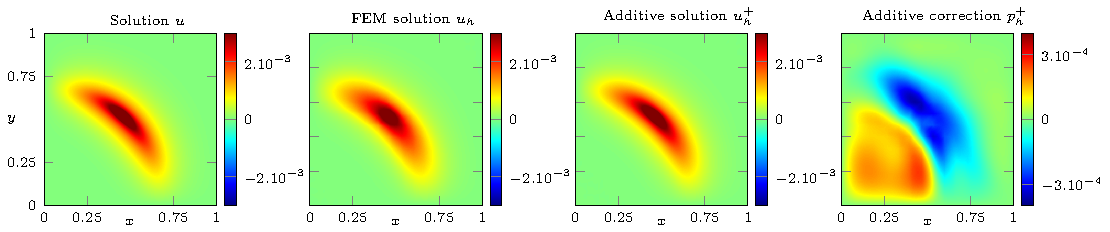
\includegraphics[width=\linewidth]{images/numeric/elliptic/plots/standalone_solutions.pdf}
		
		\vspace{8pt}
		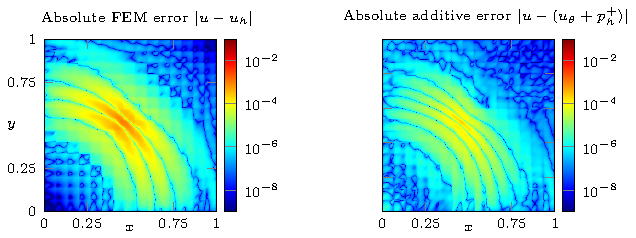
\includegraphics[width=0.7\linewidth]{images/numeric/elliptic/plots/standalone_errors.pdf}
	\end{figure}

	\vspace{-8pt}
	$$\bm{\mu}^{(2)}=(0.46,0.52,0.05,0.12)$$
\end{frame}

\subsection{2D Poisson problem on Annulus - Mixed BC}

\begin{frame}{Problem considered} 
	\textbf{Problem statement:} Considering the Poisson problem with mixed BC:
	\vspace{-5pt}
	\begin{equation*}
		\left\{
		\begin{aligned}
			-\Delta u & = f, \; &  & \text{in } \; \Omega \times \mathcal{M}, \\
			u         & = g, \;  &  & \text{on } \; \Gamma_E \times \mathcal{M}, \\
			\smash{\frac{\partial u}{\partial n}}+u  & = g_R, \;  &  & \text{on } \; \Gamma_I \times \mathcal{M},
		\end{aligned}
		\right.
		% \label{eq:Lap2DMixed}\tag{$\mathcal{P}$}
	\end{equation*}

	with $\Omega=\{(x,y)\in\mathbb{R}^2, \; 0.25\le x^2+y^2\le 1\}$ and $\mathcal{M}=[2.4,2.6]$ ($p=1$).
		
	\vspace{8pt}
	\textbf{Analytical solution :}

	\vspace{-12pt}
	\begin{equation*}
		% \label{eq:analytical_solution_Lap2D}
		u(\bm{x};\bm{\mu})= 1 - \frac{\ln\big(\mu_1\sqrt{x^2+y^2}\big)}{\ln(4)},
	\end{equation*}
	\vspace{-5pt}
	
	\textbf{Boundary conditions :}
	\begin{equation*}
		g(\bm{x};\bm{\mu})=1 - \frac{\ln(\mu_1)}{\ln(4)} \quad \text{and} \quad g_R(\bm{x};\bm{\mu})=2 + \frac{4-\ln(\mu_1)}{\ln(4)}.
	\end{equation*}

	\vspace{2pt}
	\textbf{PINN training:} MLP of 5 layers; LBFGs optimizer (4000 epochs). \\
	Imposing the mixed BC exactly in the PINN\footcite{Sukumar_2022}.

	\vspace{8pt}
\end{frame}

% \begin{frame}{Numerical results}
% 	\hspace{-5pt}\begin{minipage}[t]{0.46\linewidth}
% 		\textbf{Error estimates :} 1 set of parameters.
% 		$$\bm{\mu}^{(1)}=2.51$$
% 		\vspace{-35pt}
% 		\begin{figure}[H]
% 			\cvgFEMCorrAlldeg{images/numeric/poisson/mixed/cvg/FEM_case5_v2_param1.csv}{images/numeric/poisson/mixed/cvg/Corr_case5_v2_param1.csv}{1e-10}
% 		\end{figure}
% 	\end{minipage} \qquad \small
% 	\begin{minipage}[t]{0.48\linewidth}
% 	\end{minipage}
% \end{frame}

% \begin{frame}[noframenumbering]{Numerical results}
\begin{frame}{Numerical results}
	\hspace{-5pt}\begin{minipage}[t]{0.46\linewidth}
		\textbf{Error estimates :} 1 set of parameters.
		$$\bm{\mu}^{(1)}=2.51$$
		\vspace{-35pt}
		\begin{figure}[H]
			\cvgFEMCorrAlldeg{images/numeric/poisson/mixed/cvg/FEM_case5_v2_param1.csv}{images/numeric/poisson/mixed/cvg/Corr_case5_v2_param1.csv}{1e-10}
		\end{figure}
	\end{minipage} \qquad \small
	\begin{minipage}[t]{0.48\linewidth}
		\textbf{Gains achieved :} $n_p=50$ sets of parameters.
		$$\mathcal{S}=\left\{\bm{\mu}^{(1)},\dots,\bm{\mu}^{(n_p)}\right\}$$
		\vspace{-15pt}
		\begin{table}[H]
			\gainstableallq{images/numeric/poisson/mixed/gains/Tab_stats_case5_v2.csv}
		\end{table}

		\normalsize\centering\vspace{-20pt}
		$$h=1.33\cdot 10^{-1}$$

		\vspace{-5pt}
		Gain : $\| u-u_h\|_{L^2} / \| u-u_h^+\|_{L^2}$ \\
		\end{minipage}
\end{frame}

\begin{frame}{Numerical results}
	\begin{figure}[!ht] \centering
		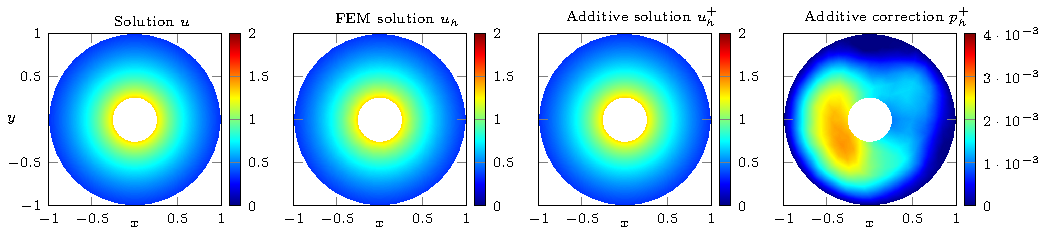
\includegraphics[width=\linewidth]{images/numeric/poisson/mixed/plots/standalone_solutions.pdf}
		
		\vspace{8pt}
		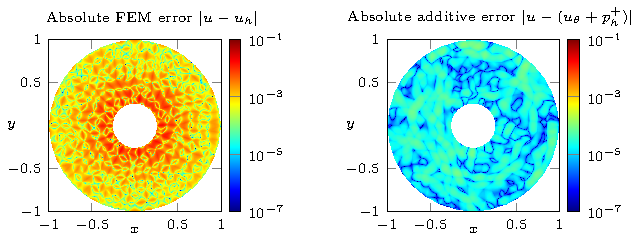
\includegraphics[width=0.7\linewidth]{images/numeric/poisson/mixed/plots/standalone_errors.pdf}
	\end{figure}

	\vspace{-8pt}
	$$\bm{\mu}^{(1)}=2.51 $$
\end{frame}